\section{薄壳结构伽辽金无网格法}

\begin{frame}{薄壳结构控制方程}

\begin{columns}
    \column{0.45\textwidth}
        \textbf{壳体中面应变与曲率}
        \begin{equation*}
            \begin{aligned}
                \epsilon_{\alpha\beta} &= \frac{1}{2}(\boldsymbol a_\alpha \cdot \boldsymbol u_{,\beta} + \boldsymbol u_{,\alpha}\cdot \boldsymbol a_\beta) \\ 
                &= \varepsilon_{\alpha\beta} + \kappa_{\alpha\beta}\xi^3 \\
            \end{aligned}
        \end{equation*}
        \textbf{Kirchhoff假设}
        \begin{equation*}
            \epsilon_{3i} = 0 \Rightarrow
            \Rightarrow \boldsymbol \theta = - \boldsymbol u_{,\alpha} \cdot \boldsymbol a_3 \boldsymbol a^\alpha
        \end{equation*}
        \vspace{-25pt}
        \begin{center}
            \tikz{\node[
                single arrow, draw,
                fill=MediumBlue,
                minimum width=0.1cm,
                minimum height=0.7cm,
                single arrow head extend=0.2cm,
                % single arrow tip angle=60,
                shape border rotate=270,
            ] {};}
        \end{center}
        \vspace{-15pt}
        \textbf{薄壳结构曲率}
        \begin{align*}
            \varepsilon_{\alpha\beta} &= \frac{1}{2}(\boldsymbol a_\alpha \cdot \boldsymbol u_{,\beta} + \boldsymbol u_{,\alpha}\cdot \boldsymbol a_\beta) \\
            \kappa_{\alpha\beta} &= (\Gamma^\gamma_{\alpha\beta}\boldsymbol u_{,\gamma} - \alert{\boldsymbol u_{,\alpha\beta}}) \cdot \boldsymbol a_3 = - \boldsymbol u_{,\alpha}\vert_\beta \cdot \boldsymbol a_3
        \end{align*}


    \column{0.5\textwidth}
        \begin{figure}
            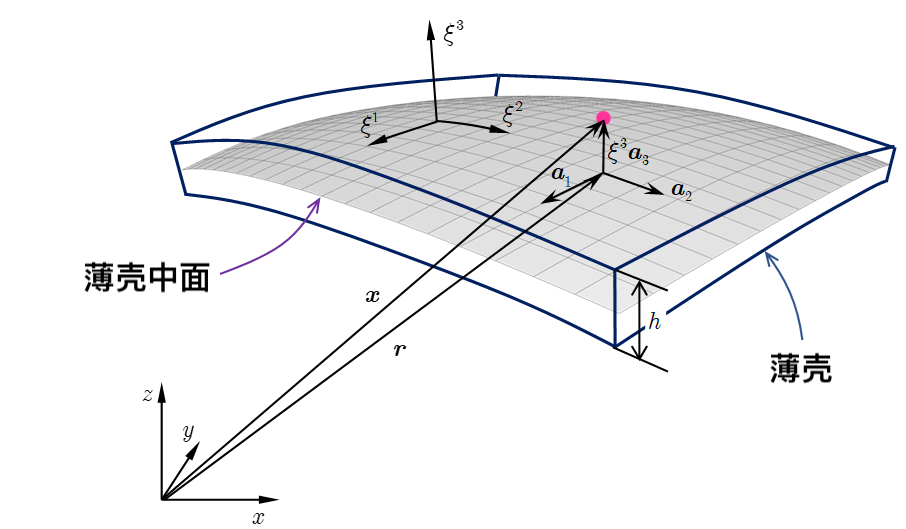
\includegraphics[width=\textwidth]{figures/1.png}
            \caption{\bfseries 薄壳结构中面}
        \end{figure}
        \begin{tcolorbox}[colback=red!5, colframe=red!75!black,left=5pt,right=5pt]
            \bfseries 薄壳结构分析曲率近似需要高阶形函数
        \end{tcolorbox}
\end{columns}

\end{frame}

\begin{frame}{再生核无网格近似}
\begin{columns}
    \column{0.45\textwidth}
        \textbf{位移近似}
        \begin{equation*}
            \boldsymbol u^h(\boldsymbol \xi) = \sum_{I=1}^{n_p} \Psi_I(\boldsymbol \xi) \boldsymbol d_I
        \end{equation*}
        \begin{equation*}
            \Psi_I(\boldsymbol \xi) = \boldsymbol p^T(\boldsymbol \xi)\boldsymbol c(\boldsymbol \xi) \phi(\boldsymbol \xi_I - \boldsymbol \xi)
        \end{equation*}
        \textbf{一致性条件}
        \begin{equation*}
            \begin{aligned}
            &\sum_{I=1}^{n_p} \Psi_I(\boldsymbol \xi)\boldsymbol p(\boldsymbol \xi_I) = \boldsymbol p(\boldsymbol \xi) \\
            \Rightarrow &
            \boldsymbol c(\boldsymbol \xi) = \boldsymbol A^{-1}(\boldsymbol \xi)\boldsymbol p(\boldsymbol 0)
            \end{aligned}
        \end{equation*}
        \textbf{无网格形函数}
        \begin{equation*}
            \Psi_I(\boldsymbol \xi) = \boldsymbol p^T(\boldsymbol \xi_I-\boldsymbol \xi) \boldsymbol A^{-1}(\boldsymbol \xi)\boldsymbol p(\boldsymbol 0)\phi(\boldsymbol \xi_I-\boldsymbol \xi)
        \end{equation*}
    \column{0.45\textwidth}
        \begin{figure}
            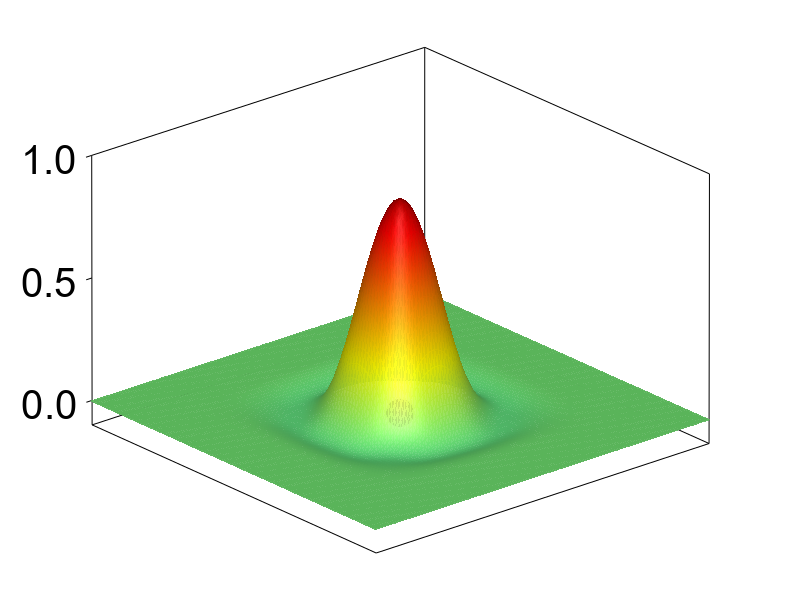
\includegraphics[width=0.7\textwidth]{figures/shape1.png}

            \vspace{-18pt}

            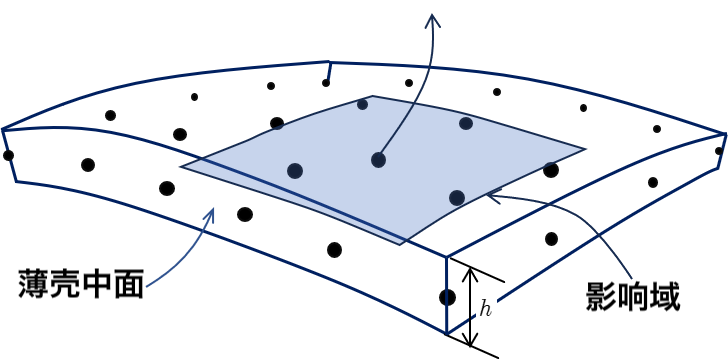
\includegraphics[width=\textwidth]{figures/3.png}
            \caption{\bfseries 再生核近似}
        \end{figure}

\end{columns}

\end{frame}

\begin{frame}{变分一致性}
\begin{columns}
    \column{0.5\textwidth}
        {\linespread{1.5}\selectfont
        \textbf{变分一致性阶次}等于伽辽金弱形式能准确求解由多项式所组成的精确解阶次:
        {\footnotesize\begin{equation*}
        \int_\Omega h \delta \varepsilon_{\alpha\beta} C^{\alpha\beta\gamma\eta} \varepsilon_{\gamma\eta}d\Omega
        +\int_\Omega \frac{h^3}{12}\delta \kappa_{\alpha\beta}C^{\alpha\beta\gamma\eta}\kappa_{\gamma\eta}d\Omega = f(\boldsymbol p^{[q]})
        \end{equation*}}
        }

    \column{0.42\textwidth}
        \begin{figure}
            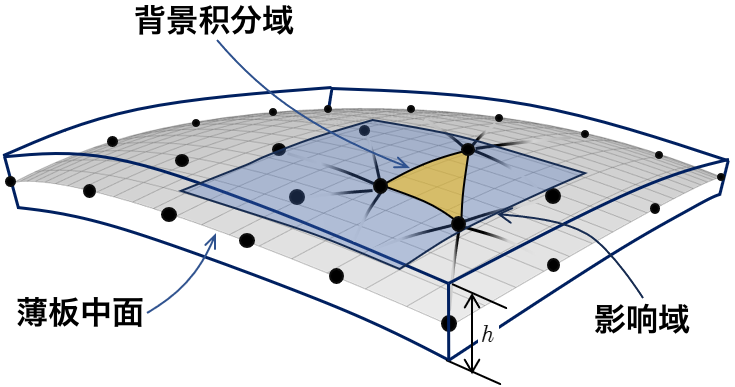
\includegraphics[width=0.9\textwidth]{figures/5.png}
            \caption{\bfseries 伽辽金无网格法数值积分}
        \end{figure}

\end{columns}

\vspace{-10pt}

\begin{tcolorbox}[colframe=MediumBlue,title=伽辽金无网格法误差估计 {\footnotesize(Wu and Wang, 2021)},height=3.4cm,valign=center]
    \begin{equation*}
    \Vert \boldsymbol u - \boldsymbol u_h\Vert_{H_e} \le \tikzmarknode[draw=red, inner sep=2pt, thick]{a}{C_p s^p\vert \boldsymbol u \vert_{H_p}} + \tikzmarknode[draw=red, inner sep=2pt, thick]{b}{C_q s^q \vert \boldsymbol u \vert_{H_q}}
    \end{equation*}
    \begin{tikzpicture}[remember picture, overlay]
        \draw[-{Stealth}, thick, red](a.south) -- ++(0,-0.3) node[below]{一致性条件控制};
        \draw[-{Stealth}, thick, red](b.north) -- ++(0,0.3) node[above]{变分一致性条件控制};
    \end{tikzpicture}

\end{tcolorbox}
\end{frame}

\begin{frame}{变分一致型边界条件施加方案}
    \begin{columns}
        \column{0.52\textwidth}
            \textbf{Nitsche法施加边界条件}

            \begin{itemize}
                \item 稳定项 \quad \uncover<2->{\alert{\footnotesize\bfseries $\times$ 人工经验参数影响求解精度}}
                    {\footnotesize\begin{equation*}
                        \begin{aligned}
                        \boldsymbol K^s_{IJ} &= \alert{\boldsymbol \alpha_v} \int_{\Gamma_v} \Psi_I \Psi_J d\Gamma 
                        + \alert{\alpha_\theta} \int_{\Gamma_\theta} \Psi_{I,\eta} n^\eta \boldsymbol a_3 \boldsymbol a_3 n^\gamma\Psi_{J,\gamma} d\Gamma \\ &+ \alert{\alpha_C} [[\Psi_I \boldsymbol a_3 \boldsymbol a_3 \Psi_J]]_{\boldsymbol x \in C_v}
                        \end{aligned}
                    \end{equation*}}
                \item 一致项 \quad \uncover<3>{\alert{\footnotesize\bfseries $\times$ 需计算形函数高阶导数}}
                    {\footnotesize\begin{equation*}
                        \begin{aligned}
                            \boldsymbol K^c_{IJ} = &- \int_{\Gamma_v} (\Psi_I \alert{\boldsymbol T_{NJ}(\Psi_{J,\alpha\beta\gamma})} + \alert{\boldsymbol T_{NI}(\Psi_{I,\alpha\beta\gamma})} \Psi_J) d\Gamma \\
                            &+ \int_{\Gamma_\theta} (\Psi_{I,\gamma} n^\gamma \boldsymbol a_3 \boldsymbol M_{\boldsymbol{nn}J} + \boldsymbol a_3 \boldsymbol M_{\boldsymbol{nn}I} \Psi_{J,\gamma}n^\gamma)d\Gamma \\
                            & + ([[\Psi_I \boldsymbol a_3 \boldsymbol P_J]] + [[\boldsymbol P_I \boldsymbol a_3 \Psi_J]])_{\boldsymbol x \in C_v}
                        \end{aligned}
                    \end{equation*}}

            \end{itemize}
        \column{0.40\textwidth}
            \begin{figure}
                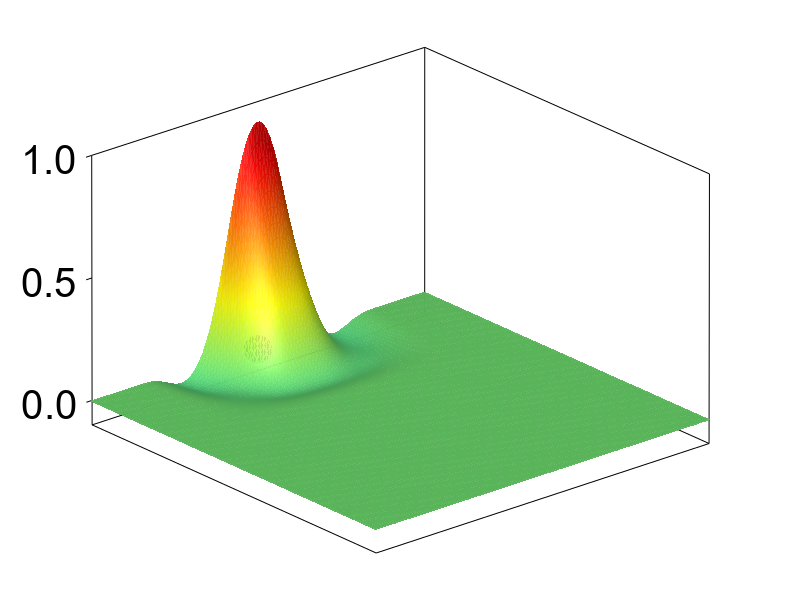
\includegraphics[width=0.7\textwidth]{figures/shape2.png}

                \vspace{-18pt}

                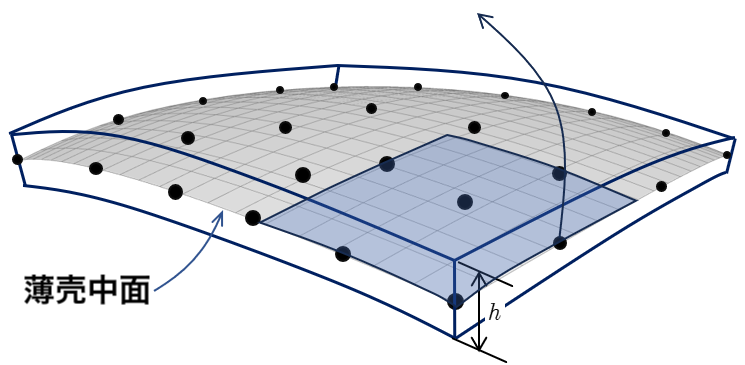
\includegraphics[width=\textwidth]{figures/4.png}
                \caption{\bfseries 边界点处无网格形函数}
            \end{figure}
    
    \end{columns}
\end{frame}

\begin{frame}{无网格形函数高阶导数}
    \begin{columns}
        \column{0.6\textwidth}
        \begin{equation*}
            \Psi_{I,ij}(\boldsymbol{\xi})=\left( \begin{aligned}
            \boldsymbol p_{,ij}^T(\boldsymbol \xi_I-\boldsymbol \xi)\boldsymbol A^{-1}(\boldsymbol \xi)\phi_s(\boldsymbol \xi_I-\boldsymbol \xi)\\
            +\boldsymbol p_{,i}^{T}(\boldsymbol \xi_I-\boldsymbol \xi)\boldsymbol A_{,j}^{-1}(\boldsymbol \xi)\phi_s(\boldsymbol \xi_I-\boldsymbol \xi)\\
            +\boldsymbol p_{,i}^{T}(\boldsymbol \xi_I-\boldsymbol \xi)\boldsymbol A^{-1}(\boldsymbol \xi)\phi_{s,j}(\boldsymbol \xi_I-\boldsymbol \xi)\\
            +\boldsymbol p^{T}(\boldsymbol \xi_I-\boldsymbol \xi)\boldsymbol A_{,ij}^{-1}(\boldsymbol \xi)\phi_s(\boldsymbol \xi_I-\boldsymbol \xi)\\
            +\boldsymbol p_{,j}^{T}(\boldsymbol \xi_I-\boldsymbol \xi)\boldsymbol A_{,i}^{-1}(\boldsymbol \xi)\phi_s(\boldsymbol \xi_I-\boldsymbol \xi)\\
            +\boldsymbol p^{T}(\boldsymbol \xi_I-\boldsymbol \xi)\boldsymbol A_{,i}^{-1}(\boldsymbol \xi)\phi_{s,j}(\boldsymbol \xi_I-\boldsymbol \xi)\\
            +\boldsymbol p^{T}(\boldsymbol \xi_I-\boldsymbol \xi)\boldsymbol A^{-1}(\boldsymbol \xi)\phi_{s,ij}(\boldsymbol \xi_I-\boldsymbol \xi)\\
            +\boldsymbol p_{,j}^{T}(\boldsymbol \xi_I-\boldsymbol \xi)\boldsymbol A^{-1}(\boldsymbol \xi)\phi_{s,i}(\boldsymbol \xi_I-\boldsymbol \xi)\\
            +\boldsymbol p^{T}(\boldsymbol \xi_I-\boldsymbol \xi)\boldsymbol A_{,j}^{-1}(\boldsymbol \xi)\phi_{s,i}(\boldsymbol \xi_I-\boldsymbol \xi)\\
           \end{aligned} \right)
            \boldsymbol p(\boldsymbol 0)
        \end{equation*}

        \column{0.38\textwidth}
            \begin{figure}
                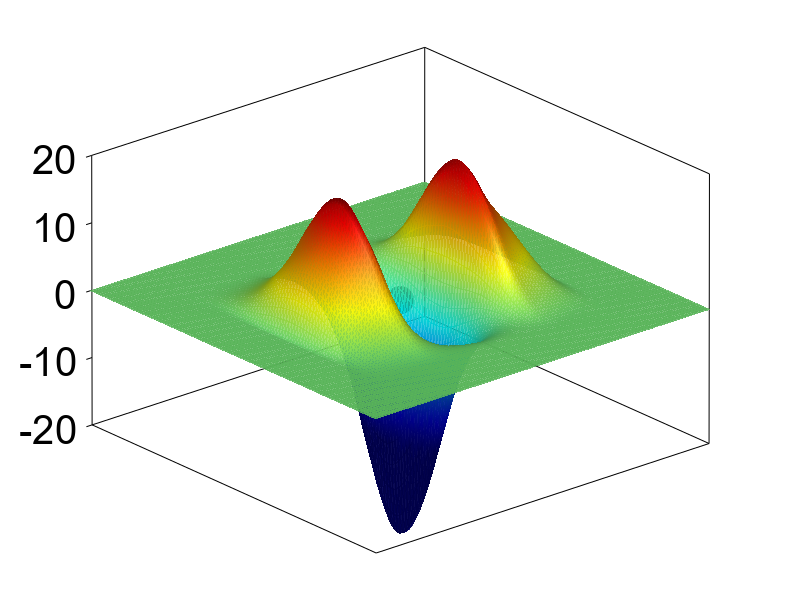
\includegraphics[width=\textwidth]{figures/shape3.png}
                \caption{\bfseries 形函数二阶导数}
            \end{figure}

            \vspace{-20pt}

            \begin{tcolorbox}[colback=red!5, colframe=red!75!black,left=5pt,right=5pt]
                \bfseries\centering 无网格形函数高阶导数\\计算复杂耗时
            \end{tcolorbox}
    \end{columns}

\end{frame}
